\RequirePackage[l2tabu, orthodox]{nag}
\documentclass{article}

\newcounter{chapter}
\setcounter{chapter}{5} % Modify Counter To Chapter

\setcounter{section}{\value{chapter}}
\addtocounter{section}{-1}

\usepackage{amssymb,amsmath,verbatim,graphicx,microtype,units,booktabs}
\usepackage[margin=10pt, font=small, labelfont=bf, labelsep=endash]{caption}
\usepackage[colorlinks=true, pdfborder={0 0 0}]{hyperref}
\usepackage[utf8]{inputenc}
\usepackage{pdfpages}

\usepackage[left=0.75in, right=0.75in]{geometry}
\usepackage{titleps}
\newpagestyle{main}{
    \setheadrule{.4pt}
    \sethead{Chapter \thechapter: \sectiontitle}
            {}
            {Illya Starikov}
}
\pagestyle{main}

\begin{document}
\section{Variations in Consciousness}
\subsection{Class Notes}
\begin{itemize}
    \item Consciousness is being aware of things occuring around self.
    \item Sleep deprived.
    \begin{itemize}
        \item Hallucinate
        \item Skin elasticity
        \item Lose color in sight
        \item Motor coordination --- wrecks will increase
        \item Immune system will go down
        \item Depression goes up
        \item Reaction time

    \end{itemize}

    \item Sleep disorders. Name five of them.
    \begin{description}
        \item [Sleep apnea] Stop breathing, \#1 cause is weight.
        \item [Insomnia]
        \begin{enumerate}
            \item Trouble falling asleep. If > 25 minutes.
            \item Trouble remaining asleep. (at least 5 or 6 hours straight)
            \item Waking up early.
        \end{enumerate}

        \item [Sleep walking] Sleep walking. Duh?
        \item [Narcoleptic] Sudden onset of sleep.
        \item [Sleep paralysis] Altered state of consciousness, not fully asleep or fully awake, where you are asleep.
        \item [RLS] Restless leg syndrome.
        \item [Night Terrors] Common in children, wake up in the middle of rem.
        \item [Enuresis] Pee the bed.
    \end{description}

    \item Why we sleep? Reboot, recharge, restore our energy.
    \item Top three dreams: Sex, being chased, falling
\end{itemize}

\subsection{Study Guide Material}
\begin{description}
    \item [EEG]
    \item [Levels of consciousness]
    \begin{itemize}
        \item Awareness of external events
        \item Awareness of internal sensations
        \item Awareness of the self as a unique being experiencing these events
        \item And awareness of your thoughts about the experiences
    \end{itemize}

    \item [Biological rhythms]
    \item [Circadian rhythms] The biological clock.
    \item [EKG] Electron-something o-gram measure brainwaves.
    \item [REM] Rapid eye movement.
    \item [Insomnia]
    \item [Narcolepsy]
    \item [Melatonin]
    \item [Sleep apnea]
    \item [Cartwright]
    \item [Freud] Said dreams were the \textit{royal road} to consciousness.
    \item [Hobson]
    \item [Mesmer]
    \item [5 stages of sleep]
    \item [sleep deprivation]
    \item [3 patterns of insomnia]
    \item [narcolepsy]
    \item [Sleep apnea]
    \item [Braid]
    \item [hypnosis]
    \item [Manta]
    \item [drugs]
    \item [Sedatives VS stimulants]
\end{description}

\subsection{Book Notes}
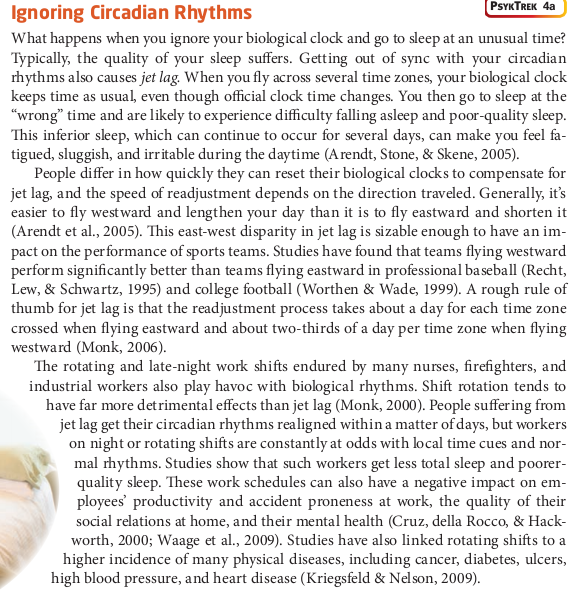
\includegraphics[width=\textwidth]{rhythm}
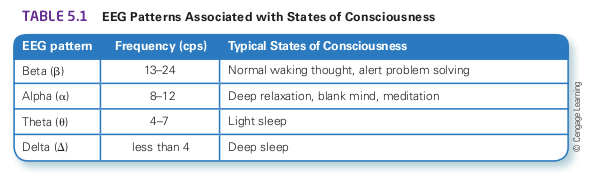
\includegraphics[width=\textwidth]{eeg}
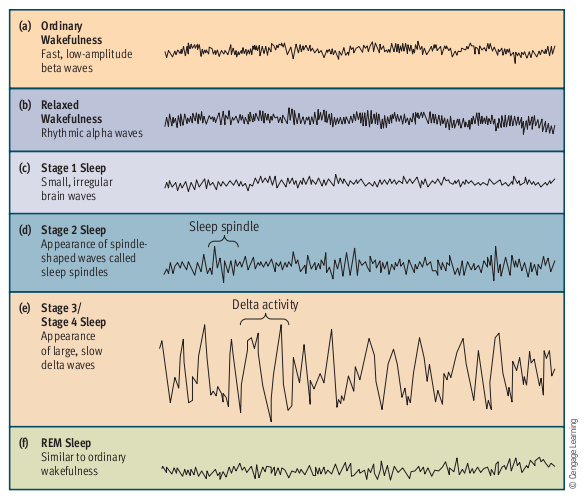
\includegraphics[width=\textwidth]{stages}

\subsection{Powerpoint Notes}
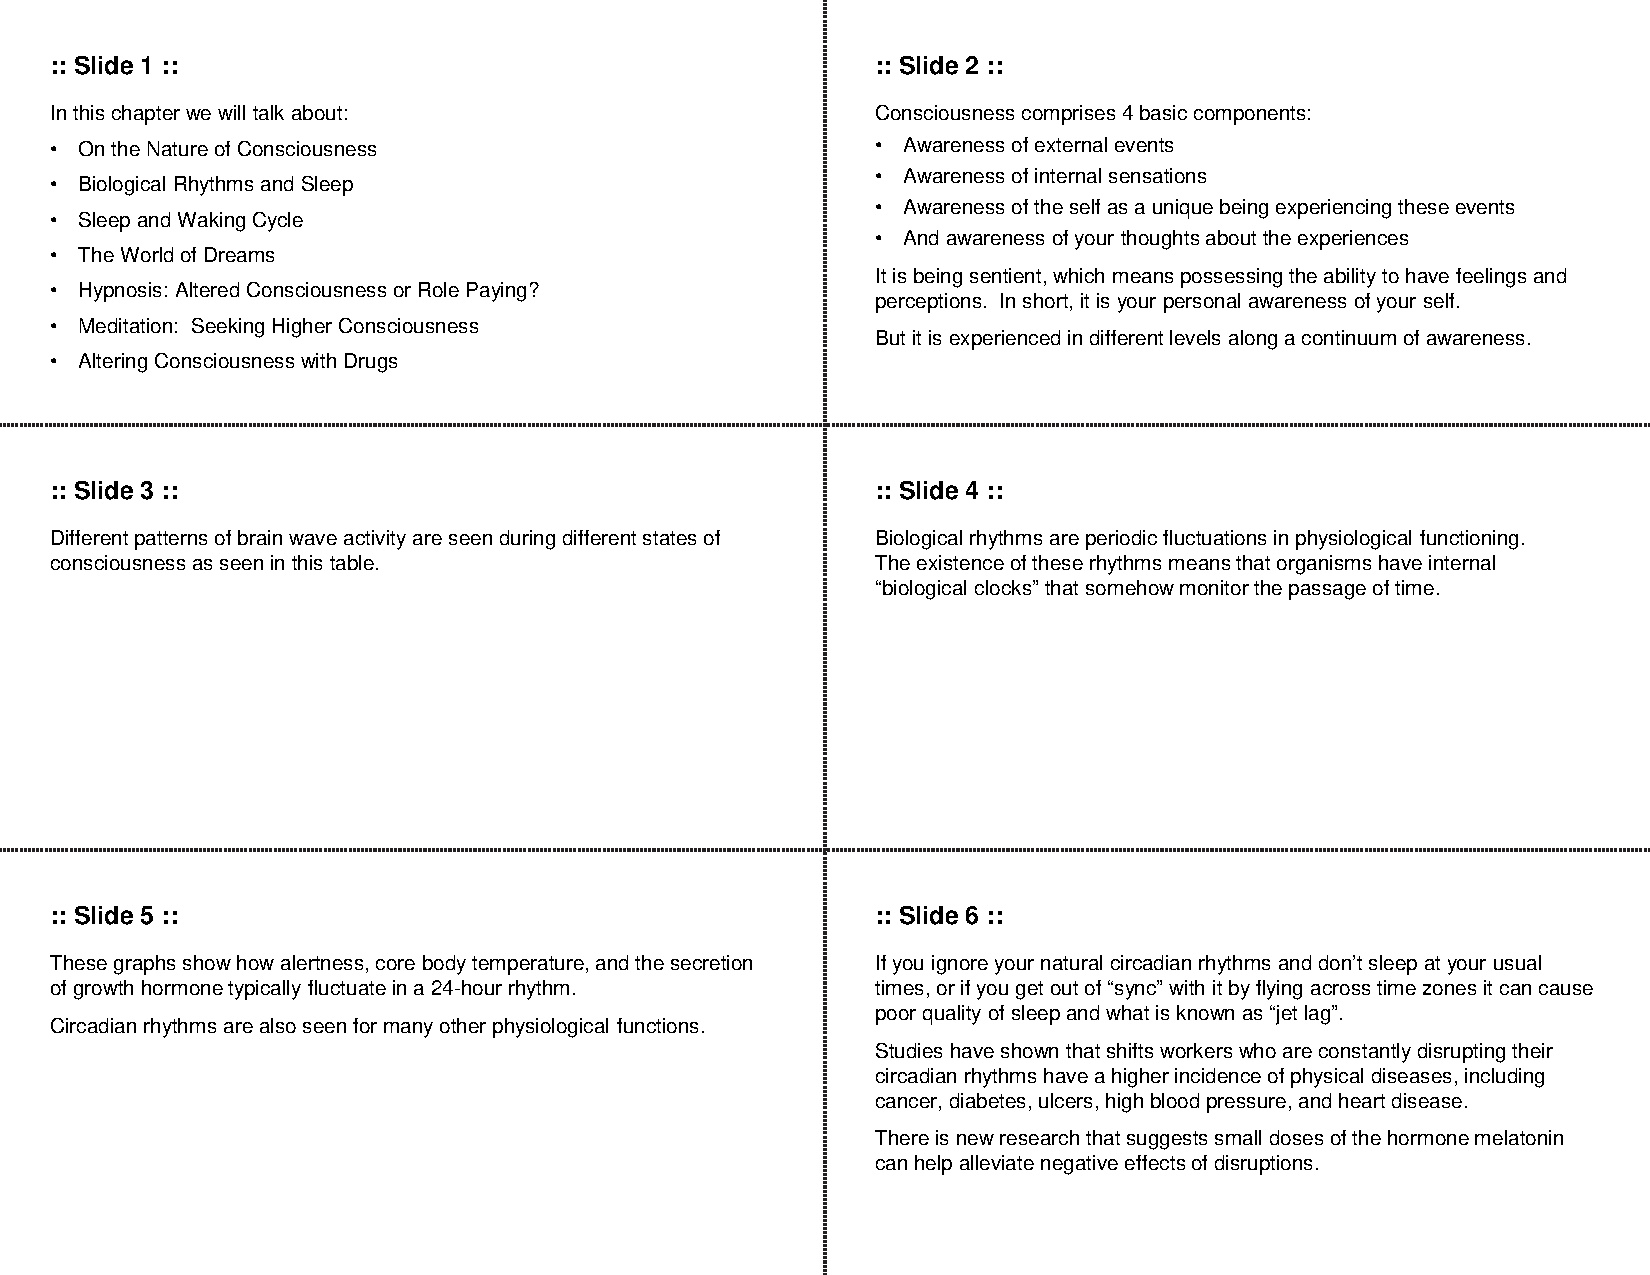
\includepdf[width=1.15\textwidth, pages=-]{lecture_notes.pdf}

\end{document}